\documentclass[tikz]{standalone}

\usepackage[T1]{fontenc}
\usepackage[english]{babel}

\usepackage{standalone}
\usepackage{graphicx}

\usetikzlibrary{calc, 3d}

\usepackage{amssymb}

\begin{document}
    \begin{tikzpicture}
        \node (model) {\includestandalone[mode=buildnew, width=2cm]{building_model}};
        \path (model.south) node[anchor=north east] (dsm) {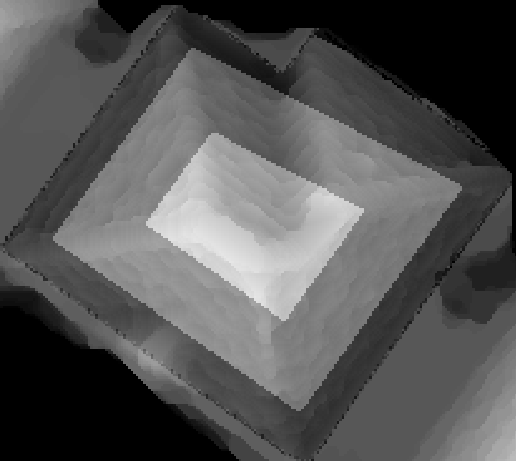
\includegraphics[width=2cm]{dsm}};
        \path (dsm.south east) node[anchor=north east] (image) {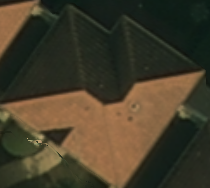
\includegraphics[width=2cm]{image}};
        
        \path (model.east |- dsm) + (1, 0) node[anchor=west] (encoder) {\includestandalone[mode=buildnew, height=6cm]{encoder}};

        \path[->, ultra thick, draw=black] (model.east) -- (encoder.west |- model);
        \path[->, ultra thick, draw=black, dashed] (dsm.east) -- (encoder.west);
        \path[->, ultra thick, draw=black, dashed] (image.east) -- (encoder.west |- image);
    \end{tikzpicture}
\end{document}
